\section{Durchführung}
\label{sec:Durchfuehrung}
\subsection{Aufnahme der Charakteristik}
Um die charakteristik des Zählrohrs aufzunehmen wird ein Beta-Strahler vor dem Zählrohr platziert und die Zählrate in Abhängigkeit von der Spannung aufgenommen.
Dabei ist zu beachten, dass der Strahler so gewählt wurde, dass die maximale Impulsrate unter 100 \sfrac{1}{\text{s}} liegt, um den effekt der Totzeit zu minimieren.
Außerdem muss die Spannung $U < 700\text{V}$ gehalten werden, damit der Zustand der Dauerentladung nicht erreicht wird.
\subsection{Totzeit}
Die Totzeit wird auf zwei Arten bestimmt.
Zum einen kann über eine Messung mit angeschlossenem Oszilloskop die Totzeit auf dem Oszilloskop abgelesen werden (Bild \ref{fig:Oszilloskop}).
\begin{figure}
    \centering
    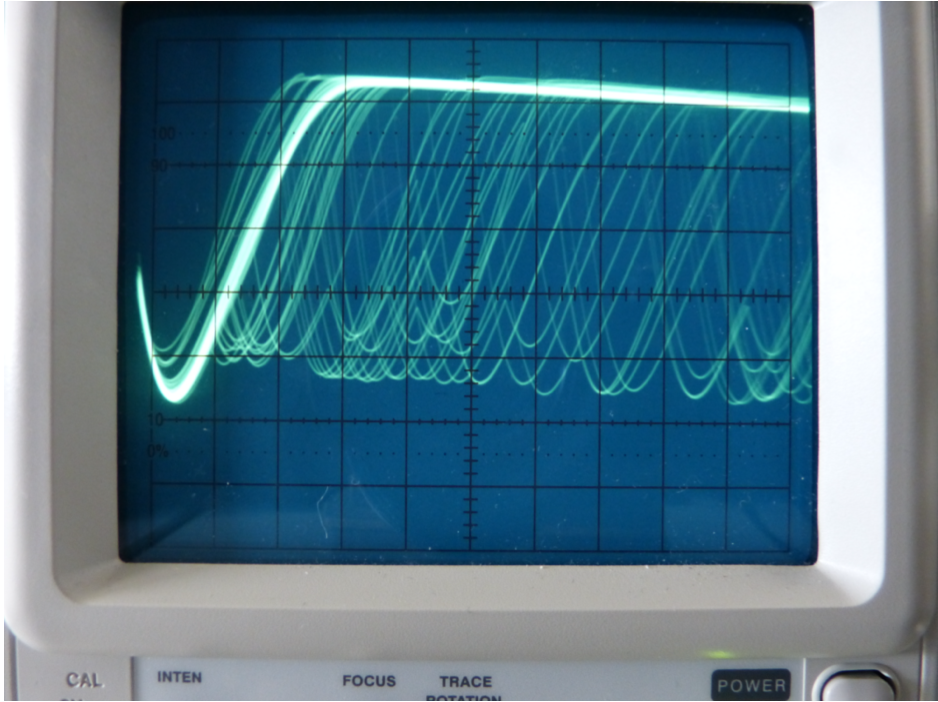
\includegraphics[width=0.5\textwidth]{bilder/Oszilloskop.png}
    \caption{Ein Ossi. (Quelle \cite{Anleitung})}
    \label{fig:Oszilloskop}
\end{figure}
Es kann aber auch über die Messung der Intensitäten zwei verschiedener Proben und der Intensität beider Proben zusammen (Bilder: \ref{sec:Anhang}) die Totzeit berechnet werden (\ref{eqn:Totzeit}).
\begin{equation}
    T_{\text{tot}} ≈ \frac{N_{1}+N_{2}-N_{1+2}}{2N_1N_2}
\end{equation}
\subsection{Ladungsmenge pro Teilchen}
Um die Ladungsmenge pro Teilchen zu bestimmen, wurde bei der Messung für Charakteristik in regelmäßigen Abständen auch der mittlere Zählstrom I gemessen.
Aus dem Zählstrom lässt sich damit die Anzahl der freigesetzten Ladungen pro Teilchen bestimmen.
\begin{equation}
    Z = \frac{I}{e_0N}
\end{equation}